\documentclass[xcolor=pdftex,dvipsnames,table]{beamer}

\usepackage{beamerthemesplit}

\setbeamertemplate{footline}[page number]{}
\setbeamertemplate{navigation symbols}{}

\definecolor{links}{HTML}{2A1B81}
\hypersetup{colorlinks,linkcolor=,urlcolor=links}

%\usepackage[colorslinks = true]{hyperref}
% set.seed(1234)

\title{Measuring Political Bias in Text with R}
\author{John Myles White}
\date{\today}

\begin{document}

\frame{\titlepage}

\frame
{
	\frametitle{Text A}
	
	\begin{quote}
		Hey, does anybody notice this crazy thing that we're on the road to socialism? I'm just saying. Wow. We got --- we got the SCHIPs thing going for us. That's great.
	\end{quote}
}

\frame
{
	\frametitle{Text B}

	\begin{quote}
		How about that McDonalds two blocks from Ground Zero? That's killed more people than the nineteen hijackers.
	\end{quote}
}

\frame
{
	\frametitle{Exploiting Artificial Artificial Intelligence}
	
	\begin{enumerate}
		\item{Text A was pro-Democrat and Text B was pro-Republican}
		\item{Text A was pro-Republican and Text A was pro-Democrat}
	\end{enumerate}
}

\frame
{
	\frametitle{Artificial Intelligence / Machine Learning}

	\begin{itemize}
		\item{People can infer political views from text}
		\item{Can computers learn to do the same?}
	\end{itemize}
}

\frame
{
	\frametitle{Desiderata}
  
 	\begin{itemize}
		\item{Continuous measure of political viewpoint}
		\item{Ability to analyze arbitrary text}
  	\end{itemize}
}

\frame
{
	\frametitle{The Ideal Points Model}
	
	\begin{itemize}
		\item{Treats politics as one dimensional}
		\item{Goes from left wing to right wing}
	\end{itemize}
}

\frame
{
	\frametitle{The Ideal Points Model}
	
	\begin{itemize}
		\item{Fit to Congressional roll call voting records}
		\item{Predicts unseen votes with $> 90\%$ accuracy}
	\end{itemize}
}

\frame
{
	\frametitle{The Ideal Points Model}
	
	\begin{itemize}
		\item{Senators have fixed positions on the scale}
		\item{Bills have fixed positions on the scale}
		\item{Senators vote ``yay'' for bills that are near their own position}
	\end{itemize}
	
	% IMAGE HERE IF POSSIBLE
}

%\frame
%{
%	\frametitle{The Ideal Points Model: Formal Bits}
%	
%	\begin{itemize}
%		\item{Senator $i$ has ideal point $\alpha_{i}$}
%		\item{Bill $j$ has ideal point $\beta_{j}$}
%		\item{Probability of ``yay`` vote is $L(\alpha - \beta)$}
%		\item{$L$ is the logistic function}
%	\end{itemize}
%}

\frame
{
	\frametitle{The Ideal Points Model}

	\begin{itemize}
		\item{Essentially logistic regression with hidden variables}
		 \item{Easy to fit using Bayesian MCMC methods}
		\item{Use JAGS through the `rjags' package}
	\end{itemize}
}


\frame
{
	\frametitle{Senate Roll Call Voting Records}

	\begin{itemize}
		\item{Available as ORD files from \href{http://voteview.com}{voteview.com}}
		\item{Read in to R using `readKH()' from `pscl' package}
	\end{itemize}
}

\frame
{
	\frametitle{Senate Roll Call Voting Records}

	\begin{itemize}
		\item{Construct roll call matrix}
		\begin{itemize}
			\item{Rows are senators}
			\item{Columns are bills}
			\item{Entries are yay / nay votes}
		\end{itemize}
		\item{Analyze data from 111th Congress}
	\end{itemize}
}

\begin{frame}[fragile]
	\frametitle{Senate Roll Call Voting Records}

	\begin{verbatim}
roll.calls <- readKH(file.path(`data',
                               `roll_calls_111.ord'))

votes <- roll.calls$votes

binary.votes <- apply(votes, c(1, 2), yes.no.vote)
	\end{verbatim}
\end{frame}

\frame
{
	\frametitle{Example Roll Call Matrix}
	
	\begin{table}[htdp]
	\begin{center}
	\rowcolors{1}{RoyalBlue!20}{RoyalBlue!5}
	\begin{tabular}{|c|c|c|c|}
	\hline
	Senator & Bill 1 & Bill 2 & Bill 3 \\
	\hline
	Byrd (D WV) & 1 & 1 & 1 \\
	Chambliss (R GA) & NA & 0 & 0 \\
	\hline
	\end{tabular}
	\end{center}
	\end{table}
}

\frame
{
	\frametitle{Using JAGS for Bayesian Inference}
	
	\begin{itemize}
		\item{Bayesian modeling gives us flexibility}
		\item{JAGS (BUGS) is a general modeling language}
		\item{JAGS lets us describe model mathematically}
		\item{JAGS compiles model into code}
		\item{Code runs MCMC and estimates model parameters}
	\end{itemize}
}

\begin{frame}[fragile]
	\frametitle{Using `rjags' to Call JAGS from R}

	\begin{verbatim}
jags <- jags.model(`jags/ideal_points.bug',
                   data = list(`votes' = binary.votes,
                               `M' = nrow(binary.votes),
                               `N' = ncol(binary.votes),
                               `a' = a),
                   n.chains = 4,
                   n.adapt = 500)

j.samples <- jags.samples(jags,
                          c(`a', `b', `g'),
                          250)
	\end{verbatim}
\end{frame}

\begin{frame}[fragile]
	\frametitle{The JAGS Model}

	\begin{verbatim}
for (i in 1:M)
{
  for (j in 1:N)
  {
    votes[i, j] ~ dbern(p[i, j])
    logit(p[i, j]) <- g[j] * (a[i] - b[j])
  }
}
	\end{verbatim}
\end{frame}

\begin{frame}[fragile]
	\frametitle{The JAGS Model}

	\begin{verbatim}
for (i in 1:M)
{
  a[i] ~ dnorm(0, tau.a)
}

tau.a <- pow(sigma.a, -2)
sigma.a ~ dunif(0, 100)
	\end{verbatim}
\end{frame}

\begin{frame}[fragile]
	\frametitle{The JAGS Model}
	
	\begin{verbatim}
for (j in 1:N)
{
  b[j] ~ dnorm(mu.b, tau.b)
  g[j] ~ dnorm(0, tau.g)
}

mu.b ~ dnorm(0, 0.0001)

tau.b <- pow(sigma.b, -2)
sigma.b ~ dunif(0, 100)

tau.g <- pow(sigma.g, -2)
sigma.g ~ dunif(0, 100)
	\end{verbatim}
\end{frame}

\frame
{
	\frametitle{Example Ideal Points for 111th Congress}
  
	\begin{table}[htdp]
	\begin{center}
	\rowcolors{1}{RoyalBlue!20}{RoyalBlue!5}
	\begin{tabular}{|l|l|}
	\hline
	Senator & Ideal Point \\
	\hline
  	Demint (R SC) & 1.79 \\
	Snowe (R SC) & 0.23 \\
	Bayh (D IN) & -0.15 \\
	Durbin (D IL) & -1.50 \\
	\hline
	\end{tabular}
	\end{center}
	\end{table}
}

\frame
{
	\frametitle{Ideal Points by Party}
	
	\begin{center}
		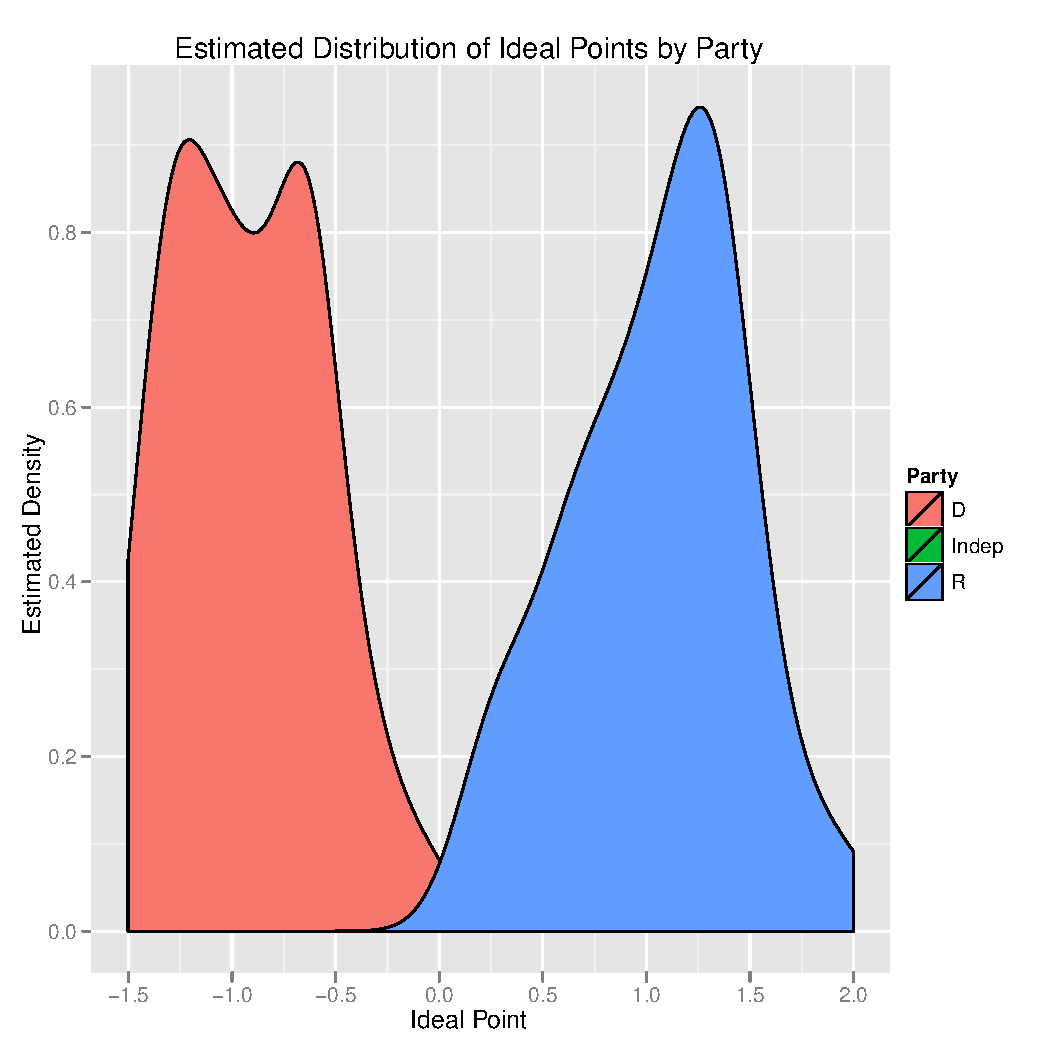
\includegraphics[scale = 0.45]{graphs/ideal_point_distribution.pdf}
	\end{center}
}

\frame
{
	\frametitle{Ideal Points: Measure of Political Bias}
	
	\begin{itemize}
		\item{Ideal points are our continuous scale for measuring bias}
		\item{How can we relate them to text?}
	\end{itemize}
}

\frame
{
	\frametitle{Harvest Congressional Text and Match with Ideal Points}
  
	\begin{itemize}
		\item{Manually gather text from each senator}
		\begin{itemize}
			\item{Floor speeches}
			\item{Press releases}
			\item{Op-eds}
		\end{itemize}
		\item{Assign senator's ideal point to text written by them}
		\item{Predict ideal points using text}
	\end{itemize}
}

\frame
{
	\frametitle{Corpus Statistics}
	
	\begin{itemize}
		\item{1,408 unique documents}
		\item{20,521 unique words}
	\end{itemize}
}

\frame
{
	\frametitle{Corpus Statistics}

	\begin{center}
		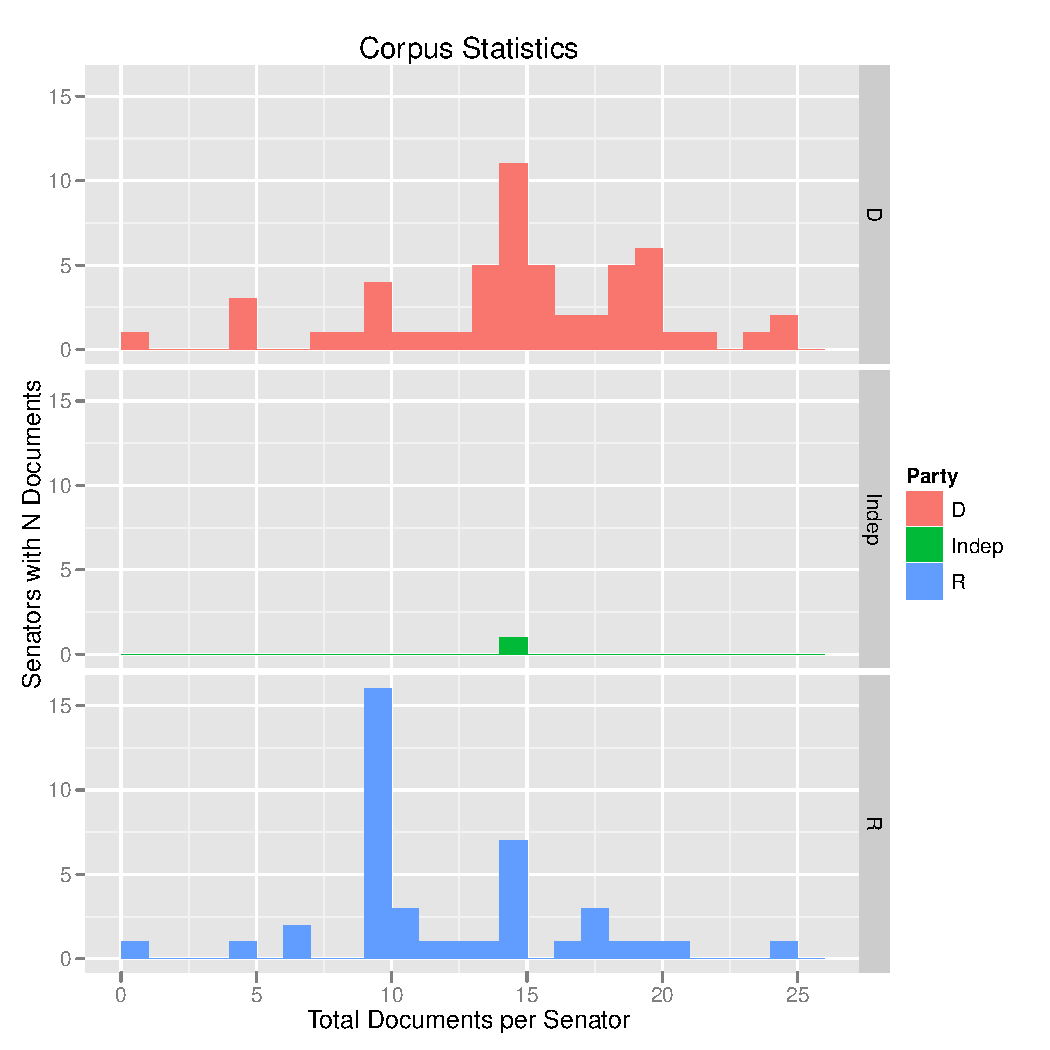
\includegraphics[scale = 0.45]{graphs/document_statistics.pdf}
	\end{center}
}

\frame
{
	\frametitle{Importing Text into R}
  
	\begin{itemize}
	  	\item{Use the `tm' package}
  		\item{Store all documents in one large CSV file}
		\item{Use `read.csv' to turn CSV file into a data.frame}
	    	\item{Create a `tm' corpus from the data.frame}
		\item{Build a document-term matrix}
	\end{itemize}
}

\frame
{
	\frametitle{Example Document A from the Corpus}
	
	\begin{quote}
	i want to talk about jobs lately it seems that everyone says they want to talk about jobs and that we'll get around to tackling jobs next week or the week after
	\end{quote}
}

\frame
{
	\frametitle{Example Document B from the Corpus}
	
	\begin{quote}
	there was a major legislative accomplishment in washington last week and it's getting less attention than it deserves because it isn't national health care reform
	\end{quote}
}

\frame
{
	\frametitle{Example Document-Term Matrix}
	
	\begin{table}[htdp]
	\begin{center}
	\rowcolors{1}{RoyalBlue!20}{RoyalBlue!5}
	\begin{tabular}{|c|c|c|c|c|c|}
	\hline
	Document & I & Want & Talk & Jobs & Week \\
	\hline
	A & 1 & 2 & 2 & 3 & 2 \\
	B & 0 & 0 & 0 & 0 & 1 \\
	\hline
	\end{tabular}
	\end{center}
	\end{table}
}

\begin{frame}[fragile]
	\frametitle{Creating a Corpus with `tm'}

	\begin{verbatim}
corpus <- Corpus(DataframeSource(documents))

corpus <- tm_map(corpus,
                 tolower)

corpus <- tm_map(corpus,
                 removeWords,
                 stopwords(`english'))
	\end{verbatim}
\end{frame}

\begin{frame}[fragile]
	\frametitle{Creating a Document Term Matrix with `tm'}

	\begin{verbatim}
document.term.matrix <- DocumentTermMatrix(corpus)

x <- as.matrix(document.term.matrix)

y <- authors$IdealPoint
	\end{verbatim}
\end{frame}

\frame
{
	\frametitle{Text Regression}

	\begin{itemize}
		\item{Turn text analysis into a standard regression problem}
		\item{Outcomes: senators' ideal points}
		\item{Predictors: document words counts}
	\end{itemize}
}

\frame
{
	\frametitle{OLS Regression: A Review}

	\begin{itemize}
		\item{Predict continuous outcome variable}
		\item{Try to minimize sum of squared errors}
		\item{Need more rows than columns}
		\item{Use `lm' or maybe `glm'}
	\end{itemize}
}

\begin{frame}[fragile]
	\frametitle{OLS Regression in R}
	
	\begin{verbatim}
x <- 1:10
y <- 3 * x + rnorm(10, 0, 1)

fit <- lm(y ~ x)

coef(fit)
	\end{verbatim}
\end{frame}

\begin{frame}[fragile]
	\frametitle{OLS Regression in R}
	
	\begin{verbatim}
(Intercept)           x 
 -0.1896415   2.9648153 
	\end{verbatim}
\end{frame}

\begin{frame}[fragile]
	\frametitle{OLS Regression in R}
	
	\begin{verbatim}
summary(fit)
	\end{verbatim}
\end{frame}

\begin{frame}[fragile]
	\frametitle{OLS Regression in R}
	
	\begin{verbatim}
Residuals:
     Min       1Q   Median       3Q      Max 
-2.01532 -0.29611 -0.06683  0.73038  1.37964 

Coefficients:
            Estimate Std. Error t value Pr(>|t|)    
(Intercept)  -0.1896     0.7174  -0.264    0.798    
x             2.9648     0.1156  25.644 5.73e-09 ***
---
Signif. codes:  0 �***� 0.001 �**� 0.01 �*� 0.05 �.� 0.1 � � 1 

Residual standard error: 1.05 on 8 degrees of freedom
Multiple R-squared: 0.988,	Adjusted R-squared: 0.9865 
F-statistic: 657.6 on 1 and 8 DF,  p-value: 5.734e-09 
	\end{verbatim}
\end{frame}

\frame
{
	\frametitle{Underdetermined Problems}

	\begin{itemize}
		\item{Fewer rows than columns}
		\item{OLS finds infinitely many solutions, all with zero error}
		\item{Need regularization to find useful solutions}
	\end{itemize}
}

\frame
{
	\frametitle{Regularized Regression}
	
	\begin{itemize}
		\item{Standard regression uses prediction error to find coefficients}
		\begin{itemize}
			\item{OLS regression}
			\item{LAD regression}
		\end{itemize}
		\item{Regularization adds a penalty for large coefficients}
		\begin{itemize}
			\item{Ridge regression (L2)}
			\item{LASSO regression (L1)}
			\item{Elastic Net regression (L2 + L1)}
		\end{itemize}
	\end{itemize}
}

\frame
{
	\frametitle{$L_{p}$ Penalities}
	
	\begin{itemize}
		\item{L2 penalty is harsh on large values}
		\item{L1 penalty is harsh on any non-zero value}
		\item{L1 induces sparse solutions}
		\item{Very few columns get non-zero coefficients}
		\item{Most columns get exactly zero coefficients}
	\end{itemize}
}

\frame
{
	\frametitle{Typical Distribution of Coefficients}

	\begin{center}
		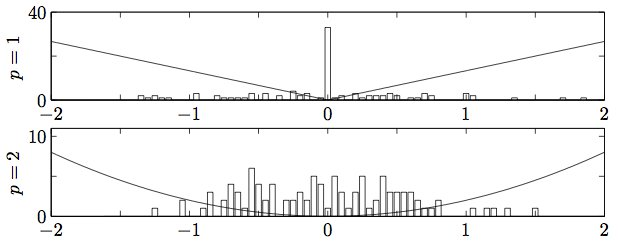
\includegraphics[scale = 0.5]{graphs/boyd.jpg}
	\end{center}
}

\frame
{
	\frametitle{Regularized Regression in R}
	
	\begin{itemize}
		\item{Use the `glmnet' package}
		\item{Fits any form of Elastic Net}
		\item{`alpha' shifts between LASSO and ridge}
		\item{`alpha'  = 1 by default, which gives LASSO}
		\item{`lambda' controls the prediction error / regularization tradeoff}
		\item{`glmnet' fits many values of `lambda'  automatically}
	\end{itemize}
}

\begin{frame}[fragile]
	\frametitle{Simple glmnet Example}
	
	\begin{verbatim}
x1 <- c(1, 2, 3)
x2 <- c(1, 1, 3)
x3 <- c(1, 4, 3)
x <- cbind(x1, x2, x3)

a <- 1
b <- 2
c <- 3
	
y <- a * x1 + b * x2 + c * x3 + rnorm(3, 0, 1)
	\end{verbatim}
\end{frame}

\begin{frame}[fragile]
	\frametitle{Simple glmnet Example}

	\begin{verbatim}
library(`glmnet')

fit <- glmnet(x, y)

fit
	\end{verbatim}
\end{frame}

\begin{frame}[fragile]
	\frametitle{Simple glmnet Example}

	\begin{verbatim}
Call:  glmnet(x = x, y = y) 

      Df   %Dev Lambda
 [1,]  0 0.0000 4.3300
 [2,]  1 0.1550 3.9460
...
[38,]  2 0.9989 0.1385
[39,]  2 0.9991 0.1262
	\end{verbatim}
\end{frame}

%\begin{frame}[fragile]
%	\frametitle{Simple glmnet Example}
%
%	\begin{verbatim}
%coef(fit, s = 0)
%coef(fit, s = 1)
%coef(fit, s = 2)
%	\end{verbatim}
%\end{frame}

\frame
{
	\frametitle{Out of Sample Model Validation}
	
	\begin{itemize}
		\item{Don't want to overfit data}
		\item{Assess final model on data not used during model fitting}
		\item{Split data into two parts: training set and test set}
		\item{2 / 3 of data goes into training set}
		\item{1 / 3 of data goes into test set}
	\end{itemize}
}

\begin{frame}[fragile]
	\frametitle{Training Set / Test Set Split}
	
	\begin{verbatim}
training.size <- round(length(y) * (2 / 3))
test.size <- round(length(y) * (1 / 3))

training.indices <- sample(1:length(y), training.size)

training.x <- x[training.indices, ]
training.y <- y[training.indices]
test.x <- x[!test.indices, ]
test.y <- y[!test.indices]
	\end{verbatim}
\end{frame}

%\frame
%{
%	\frametitle{Regularization, Hyperparameters and Overfitting}
%	
%	\begin{itemize}
%		\item{`lambda' hyperparameter controls overfitting vs. underfitting}
%		\item{Can't set `lambda' using naive prediction error on training set}
%		\item{Need another approach for setting hyperparameters}
%	\end{itemize}
%}

\frame
{
	\frametitle{Back to `lambda'}
	
	\begin{itemize}
		\item{If `lambda' = 0, get OLS regression results}
		\item{Zero prediction error, but model is meaningless}
		\item{If `lambda' = $\infty$, coefficients go to zero}
		\item{Model predicts the same outcome for all rows}
		\item{Need to find sweet spot}
	\end{itemize}
}

\frame
{
	\frametitle{Hyperparameter Tuning}
  
	\begin{itemize}
		\item{Split training set into fitting subset and assessment subset}
		\item{Repeat splitting process many times}
		\item{Calculate error for many `lambda' values}
		\item{Pick `lambda' with lowest average out-of-sample error}
	\end{itemize}
}

%\frame
%{
%	\frametitle{Performance Loop}
%	
%	Split data
%	Fit Model
%	Test Model
%	Store results
%}

\frame
{
	\frametitle{Example Model Performance Table}

\begin{table}[htdp]
\rowcolors{1}{RoyalBlue!20}{RoyalBlue!5}
\begin{center}
\begin{tabular}{|c|c|c|}
\hline
Iteration & Lambda & RMSE \\
\hline
1 & 1 & 1.03 \\
2 & 1 & 1.07 \\
1 & 0.5 & 0.98 \\
2 & 0.5 & 0.99 \\
\hline
\end{tabular}
\end{center}
\label{default}
\end{table}
}

\begin{frame}[fragile]
	\frametitle{Hyperparameter Tuning}

	\begin{verbatim}
mean.rmse <- ddply(performance, `Lambda', mean)

min.rmse <- with(mean.rmse, min(RMSE))

optimal.lambda <- with(subset(mean.rmse,
                              RMSE == min.rmse),
                       Lambda)
	\end{verbatim}
\end{frame}

\frame
{
	\frametitle{The ..ply functions from `plyr'}
	
	\begin{itemize}
		\item{Split, apply, combine strategy}
		\item{Specify initial data.frame}
		\item{Specify columns to use to split data}
		\item{Specify function to apply to subsets}
		\item{Returns combined results from all subsets}
	\end{itemize}
}

\begin{frame}[fragile]
	\frametitle{ddply Example}
	
	\begin{verbatim}
df <- data.frame(Class = c(1, 1, 2, 2),
	                 Score = c(10, 15, 20, 25))
	
ddply(df, `Class', function (df) {with(df, mean(Score))})
	\end{verbatim}
\end{frame}

\begin{frame}[fragile]
	\frametitle{ddply Example}
	
	\begin{verbatim}
  Class   V1
1     1 12.5
2     2 22.5
	\end{verbatim}
\end{frame}

\frame
{
	\frametitle{Hyperparameter Tuning Results}
	
	\begin{center}
		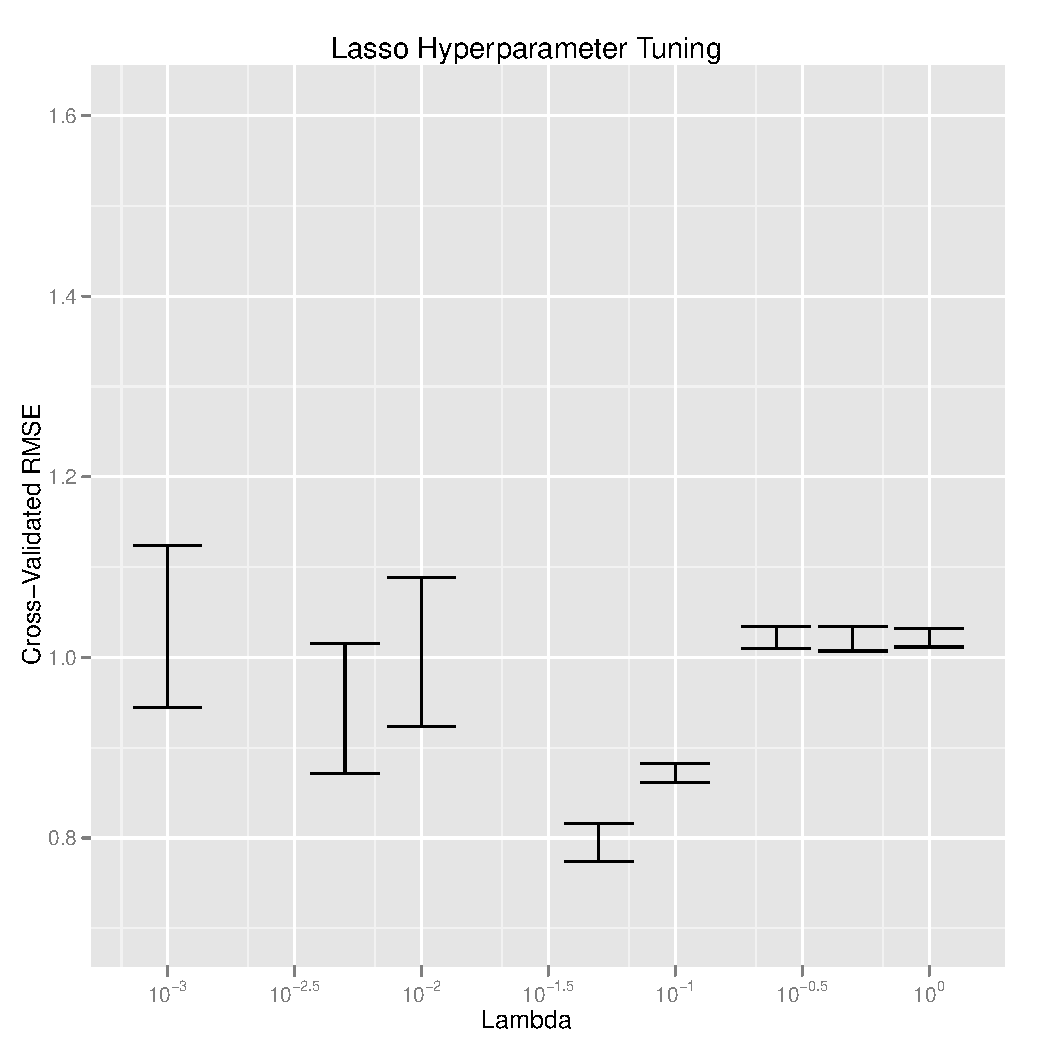
\includegraphics[scale = 0.45]{graphs/lambda_rmse.pdf}
	\end{center}
}


\begin{frame}[fragile]
	\frametitle{Fit Final Model}
	
	\begin{verbatim}
fit <- glmnet(training.x, training.y)
	\end{verbatim}
\end{frame}

\begin{frame}[fragile]
	\frametitle{Find Most Biased Terms}

	\begin{verbatim}

term.weights <- coef(fit, s = optimal.lambda)

sorted.terms <- sort(term.weights[,1])

n <- length(sorted.terms)

most.democratic.terms <- sorted.terms[1:10]
most.republican.terms <- sorted.terms[(n - 9):n]
	\end{verbatim}
\end{frame}

\frame
{
\frametitle{Top 10 Most Republican Terms}

\begin{table}[htdp]
\rowcolors{1}{RoyalBlue!20}{RoyalBlue!5}
\begin{center}
\begin{tabular}{|c|c|}
\hline
Term & Value \\ 
\hline
okla & 1.23 \\
bailey & 0.647 \\
johnny & 0.588 \\
administering & 0.561 \\
neb & 0.556 \\
sam & 0.542 \\
986 & 0.532 \\
texans & 0.493 \\
patriotism & 0.466 \\
demint & 0.417 \\
\hline
\end{tabular}
\end{center}
\label{default}
\end{table}
}

\frame
{
\frametitle{Top 10 Most Democratic Terms}

\begin{table}[htdp]
\rowcolors{1}{RoyalBlue!20}{RoyalBlue!5}
\begin{center}
\begin{tabular}{|c|c|}
\hline
Term & Value \\ 
\hline
sherrod & -0.367 \\
sheldon & -0.249 \\
dec & -0.196 \\
possess & -0.168 \\
salaries & -0.158 \\
tom & -0.152 \\
debbie & -0.151 \\
dark & -0.148 \\
lautenberg & -0.133 \\
fought & -0.106 \\
\hline
\end{tabular}
\end{center}
\label{default}
\end{table}
}

\frame
{
\frametitle{Debugging Our Results}

\begin{itemize}
	\item{Too many names of senators in our list}
	\item{Strip out all the names from corpus}
	\item{Run analysis from scratch on clean corpus}
\end{itemize}
}

\frame
{
\frametitle{Top 10 Most Republican Terms excluding Names}

\begin{table}[htdp]
\rowcolors{1}{RoyalBlue!20}{RoyalBlue!5}
\begin{center}
\begin{tabular}{|c|c|}
\hline
Term & Value \\ 
\hline
okla & 1.13 \\
neb & 0.726 \\
bailey & 0.674 \\
2415 & 0.638 \\
986 & 0.578 \\
kansans & 0.543 \\
administering & 0.516 \\
texans & 0.467 \\
profoundly & 0.459 \\
patriotism & 0.430 \\
\hline
\end{tabular}
\end{center}
\label{default}
\end{table}
}

\frame
{
\frametitle{Top 10 Most Democratic Terms excluding Names}

\begin{table}[htdp]
\rowcolors{1}{RoyalBlue!20}{RoyalBlue!5}
\begin{center}
\begin{tabular}{|c|c|}
\hline
Term & Value \\ 
\hline
cedar & -0.224 \\
chaired & -0.197 \\
dec & -0.158 \\
dark & -0.146 \\
blocked & -0.138 \\
reverses & -0.134 \\
1960s & -0.125 \\
insurers & -0.0958 \\
fought & -0.0926 \\
possess & -0.0923 \\
\hline
\end{tabular}
\end{center}
\label{default}
\end{table}
}

\begin{frame}[fragile]
\frametitle{Assessing Our Predictive Power}

	\begin{verbatim}
predicted.y <- predict(fit,
                       newx = test.x,
                       s = optimal.lambda)

predicted.y <- as.numeric(predicted.y[,1])

predictions <- data.frame(Predicted = predicted.y,
                          Empirical = test.y,
                          Residual = predicted.y - test.y)
	\end{verbatim}
\end{frame}

\begin{frame}[fragile]
\frametitle{Assessing Our Predictive Power}

	\begin{verbatim}
RMSE <- with(predictions, sqrt(mean(Residual ^ 2)))
	\end{verbatim}
\end{frame}

\frame
{
\frametitle{Final Model Comparison Results}
  
\begin{table}[htdp]
\rowcolors{1}{RoyalBlue!20}{RoyalBlue!5}
\begin{center}
\begin{tabular}{|c|c|}
\hline
Model & RMSE \\
\hline
Pure Intercept Regression & 1.02 \\
Lasso Text Regression excluding Senators' Names & 0.879 \\
Lasso Text Regression including Senators' Names & 0.805 \\
\hline
\end{tabular}
\end{center}
\label{default}
\end{table}
}


%# Other Figures Tables
%Ideal Points Distributions
%Number of Documents per Senator
%Most Democratic Terms
%Most Republican Terms
%Most Democratic Terms without Names
%Most Republican Terms without Names
%RMSE Table
%Cross-Validation Plot

\frame
{
	\frametitle{CRAN Packages Used}
	
	\begin{itemize}
		\item{\href{http://cran.r-project.org/web/packages/pscl/index.html}{pscl}}
		\item{\href{http://cran.r-project.org/web/packages/rjags/index.html}{rjags}}
		\item{\href{http://cran.r-project.org/web/packages/plyr/index.html}{plyr}}
		\item{\href{http://cran.r-project.org/web/packages/ggplot2/index.html}{ggplot2}}
		\item{\href{http://cran.r-project.org/web/packages/glmnet/index.html}{glmnet}}
		\item{\href{http://cran.r-project.org/web/packages/ProjectTemplate/index.html}{ProjectTemplate}}
	\end{itemize}
}

\frame
{
  \frametitle{Links}
  
  \begin{itemize}
    \item{\href{http://github.com/johnmyleswhite/senate_analyses}{Senate Analyses on GitHub}}
    \item{\href{http://ideologicalcartography.com}{Adam Bonica's Blog}}
    \item{\href{http://jackman.stanford.edu/mcmc/index.php}{Simon Jackman's Bayes Page}}
    \item{\href{http://www.cs.cmu.edu/~nasmith/}{Noah Smith's CMU Page}}
    \item{\href{http://www.cs.princeton.edu/~blei/}{David Blei's Princeton Page}}
    \item{\href{http://johnmyleswhite.com}{My Blog}}
  \end{itemize}
}

\end{document}
